\documentclass[../main.tex]{subfiles}

\begin{document}

\subsection{Aim 1: Creation of Gold Standard Clinical Trials Data Set}

The NLP tasks involved in transforming eligibility criteria into database queries may include \textbf{named entity recognition} (NER) to tag meaningful spans of text as named entities, \textbf{relation extraction} to classify relations between named entities, \textbf{normalization} to map named entities to common coded representations (e.g., ICD-10), \textbf{negation detection} to detect negated statements (e.g., "not hypertensive") and so on. Gold standard corpora quality can thus directly affect performance and the validation of each of these tasks. Such corpora can serve as reliable benchmarks for purposes of comparing NLP methods as well as training data sets. 

In Aim 1 we aim to create a gold standard corpus of human-annotated clinical trial eligibility criteria. Predictive models trained on this corpus enable and are used in subsequent Aims of this project. This aim is complete and was published in August 2022 \cite{dobbins2019leaf}.

\subsubsection{Related Work}

A number of corpora related to clinical trials have been published \cite{kury2020chia, kang2017eliie, weng2011elixr, yu2020}. Weng \textit{et al} developed EliXR \cite{weng2011elixr}, a rule-based information extraction (IE) pipeline and corpus of 1,000 eligibility criteria documents for NER and relation extraction. The corpus was not made publicly available. Kang \textit{et al} created an annotation schema based on the Observational Medical Outcomes Partnership (OMOP) Common Data Model \cite{hripcsak2015observational} and an annotated corpus of 230 eligibility criteria documents, though the corpus focused narrowly on Alzheimer's Disease-related trials only \cite{kang2017eliie}. More recently, Kury \textit{et al} created Chia \cite{kury2020chia}, a publicly available corpus of 1,000 Phase IV trials similarly focused on the OMOP Common Data model but across a variety of disease domains and with a greater number of types of entities and relations. Yu \textit{et al} \cite{yu2020} released a corpus designed for direct text-to-query generation with semantic parsing, however given the relative simplicity of generated queries to date compared to the complexity of clinical databases, it is not clear this approach is yet viable for real-world clinical trials recruitment.

\subsubsection{Eligibility Criteria and Database Queries}
The NLP tasks involved in transforming eligibility criteria into database queries include \textbf{named entity recognition} (NER) to tag meaningful spans of text as named entities, \textbf{relation extraction} to classify relations between named entities, \textbf{normalization} to map named entities to common coded representations (e.g., ICD-10), \textbf{negation detection} to detected negated statements (e.g., "not hypertensive") and so on. Gold standard corpora quality can thus directly affect performance and the validation of each of these tasks. Figure \ref{aim1_fig_lct_text2sql} illustrates why corpora structure and integrity are important for the task of query generation, using examples of eligibility criteria annotated using the LCT annotation schema and corresponding hypothetical Structured Query Language (SQL) queries. In the first eligibility criterion, "preeclampsia" is explicitly named, and thus can be directly normalized to an ICD-10 or other coded representation. However, eligibility criteria involving non-specific drugs, conditions, procedures, contraindications, and so on are used frequently in clinical trials. In the second criterion in Figure \ref{aim1_fig_lct_text2sql}, "diseases" in "diseases that affect respiratory function" is non-specific, and must be reasoned upon in order to determine appropriate codes, such as asthma, chronic obstructive pulmonary disease (COPD), or emphysema.  Programmatically reasoning to generate queries in such cases would be challenging and often impossible if the underlying semantics were not captured appropriately. With this in mind, we developed the LCT annotation schema in order to enable reasoning and ease query generation for real-world clinical trials use. As the second example in Figure \ref{aim1_fig_lct_text2sql} shows, the LCT annotation captures the semantics of complex criteria, with changes to "respiratory function" annotated using a \textit{Stability[change]} entity and \textit{Stability} relation, and the cause, "diseases" annotated with a \textit{Caused-By} relation.

\begin{figure}[h!]
  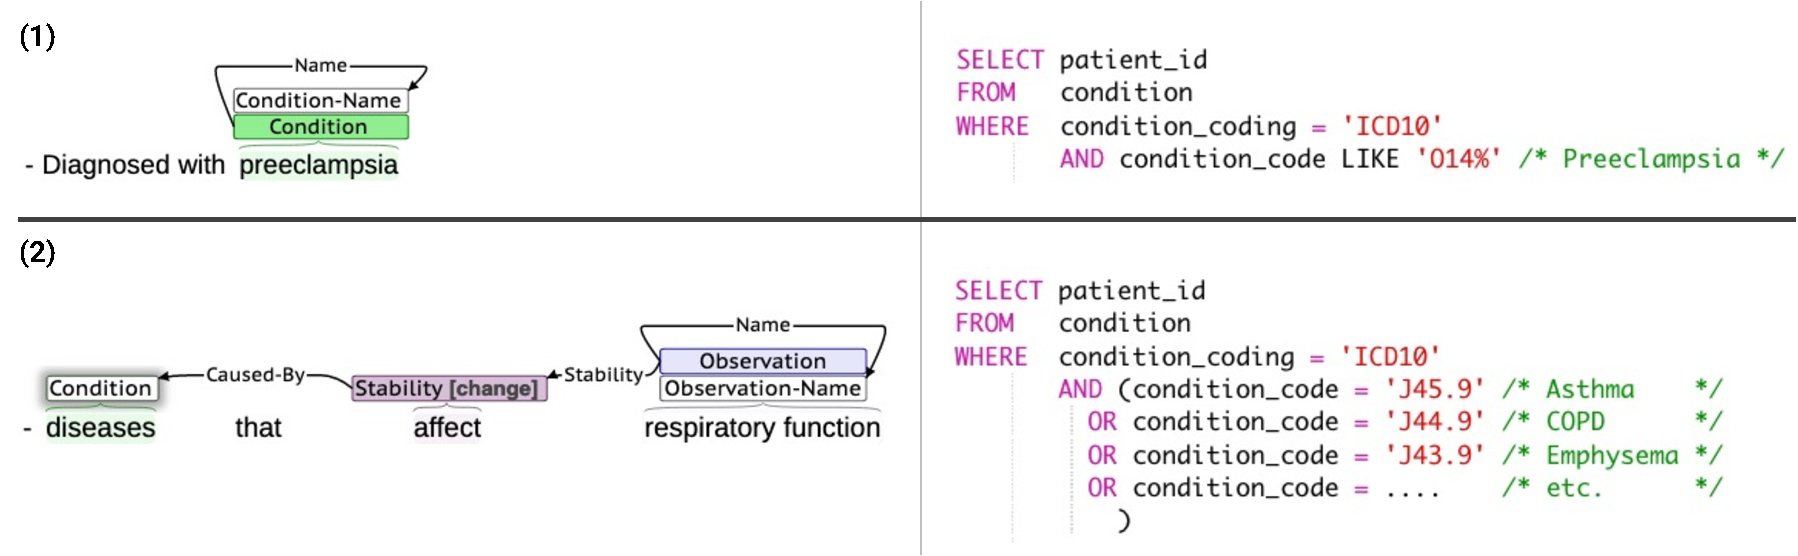
\includegraphics[scale=0.57]{Figures/Aim1/aim1_lct_text2sql.pdf}  
  \caption{Example eligibility criteria annotated used the LCT corpus annotation schema (left) and corresponding example SQL queries (right) using a hypothetical database table and columns. Annotations were done using the Brat annotation tool \cite{stenetorp2012brat}. The ICD-10 codes shown are examples and not intended to be exhaustive.}
  \label{aim1_fig_lct_text2sql}
\end{figure}

\subsubsection{Annotation schema}

We aimed to develop an expressive, task-oriented annotation schema which could capture a wide range of medical concepts and logical constructs present in eligibility criteria. To accomplish this, we first analyzed previously published corpora \cite{weng2011elixr,boland2012elixrtime,kang2017eliie,kury2020chia} and expanded the list of included biomedical phenomena to fully capture the context and logic present in real clinical trials criteria. As one example, we introduced an entity called \textit{Contraindication} to reflect where use of a given treatment is inadvisable due to possible harm to the patient. 

The LCT annotation schema is designed with the following goals and assumptions:

\begin{enumerate}
    \item The annotation schema should be \textbf{practical} and  \textbf{task-oriented} with a focus on facilitating ease of query generation. 
    \item A greater number of \textbf{more specific}, \textbf{less ambiguous} annotated phenomena should be favored over a smaller number of possibly ambiguous ones.
    \item Annotations should be \textbf{easily transformable} into composable, interconnected programmatic objects, trees, or node-edge graph representations.
    \item The annotation schema should \textbf{model eligibility criteria intent and semantics} as closely as possible in order to ensure generated queries can do the same.
\end{enumerate}

The LCT annotation schema is composed of \textbf{entities} and 
\textbf{relations}. Entities refer to biomedical, demographic, or other named entities relevant to eligibility criteria, and are annotated as a span of one or more tokens. We organized LCT entities into the following categories:

\begin{itemize}
    \item \textbf{Clinical} - \textit{Allergy, Condition, Condition-Type, Code, Contraindication, Drug, Encounter, Indication, Immunization, Observation, Organism, Specimen, Procedure, Provider}. %14
    \item \textbf{Demographic} - \textit{Age, Birth, Death, Ethnicity, Family-Member, Language, Life-Stage-And-Gender}. %21
    \item \textbf{Logical} - \textit{Exception, Negation}. %23
    \item \textbf{Qualifiers} - \textit{Acuteness, Assertion, Modifier, Polarity, Risk, Severity, Stability}. %30
    \item \textbf{Comparative} - \textit{Criteria-Count, Eq-Comparison} (an abbreviation of "Equality Comparison"), \textit{Eq-Operator, Eq-Temporal-Period, Eq-Temporal-Recency, Eq-Temporal-Unit, Eq-Unit, Eq-Value}. %38
    \item \textbf{Other} - \textit{Coreference, Insurance, Location, Other, Study}. %43
\end{itemize}

The LCT corpus also includes 7 \textit{Name} entities: \textit{Allergy-Name}, \textit{Condition-Name}, \textit{Drug-Name}, \textit{Immunization-Name}, \textit{Observation-Name}, \textit{Organism-Name} and \textit{Procedure-Name}. \textit{Name} entities serve a special purpose in the LCT corpus, as they indicate that a span of text refers to a \textit{specific} condition, drug, etc., as opposed to \textit{any} condition or drug. \textit{Name} entities overlap with their respective general entities. For example, the span "preeclampsia" refers to a specific condition, and would thus be annotated as both a \textit{Condition} and \textit{Condition-Name}, while the span "diseases" is non-specific and would be annotated as only \textit{Condition}. A full listing of the LCT annotation guidelines can be found at \url{https://github.com/uw-bionlp/clinical-trials-gov-annotation/wiki}.

We defined a total of 50 entities in the LCT corpus. In our representation, a subset of entities have \textbf{values} as well. For example, an \textit{Encounter} may have a value of \textit{emergency}, \textit{outpatient} or \textit{inpatient}. Values are optional in some entities (such as \textit{Encounters} or \textit{Family-Member}, where they may not always be clear or are intentionally broad) and always present in others. In the example annotations presented below, values are denoted using brackets ("[...]") following entity labels.

Relations serve as semantically meaningful connections between entities, such as when one entity acts upon, is found by, caused by, or related in some way to another. We categorize relations into the following:

\begin{itemize}
    \item \textbf{Alternatives and Examples} - \textit{Abbrev-Of, Equivalent-To, Example-Of}. %3
    \item \textbf{Clinical} - \textit{Code, Contraindicates, Indication-For, Name, Provider, Specimen, Stage, Type}. %10
    \item \textbf{Dependent} - \textit{Caused-By, Found-By, Treatment-For, Using}. %14
    \item \textbf{Logical} - \textit{And, If-Then, Negates, Or}. %18
    \item \textbf{Qualifier} - \textit{Acuteness, Asserted, Dose, Modifies, Polarity, Risk-For, Severity, Stability}.
    \item \textbf{Comparative} - \textit{After, Before, Criteria, Duration, During, Max-Value, Min-Value, Minimum-Count, Numeric-Filter, Operator, Per, Temporal-Period, Temporal-Recency, Temporal-Unit, Temporality, Unit, Value}.
    \item \textbf{Other} - \textit{From, Except, Has, Is-Other, Location, Refers-To, Study-Of}.
\end{itemize}

\noindent We defined a total of 51 relations in the LCT corpus.

In our annotations, some entity spans overlap with other entity spans in order to fully capture complex underlying semantics. Consider for example, the expression "Ages 18-55 years old". While an \textit{Age} entity may be assigned to token "Ages", if an \textit{Eq-Comparison} entity alone were assigned to the span "18-55 years old", the underlying semantics of the tokens "18", "-", "55", and "years" would be lost. In the following examples, we use the term \textbf{fine-grained entity} to refer to entities which are sub-spans of other \textbf{general entities}. Fine-grained entities are linked to general entities by relations. We use down arrow symbols (↓) to denote entity annotation and left and right arrow symbols (← and →) to denote relations. The (+) symbols denote overlapping entities on the same span.

The example expression "Ages 18-55 years old" would be annotated in three layers. In the first layer, the expression is annotated with \textit{Age} and \textit{Eq-Comparison} general entities with a relation between them: \\

\begin{center}
\begin{tabular}{c c c c c c c}
    "Ages" & & \multicolumn{5}{c}{$\underbrace{\text{"18 \, \, - \, \, 55 \, \, years \, \, old"}}$} \\ 
    \big\downarrow & & \multicolumn{5}{c}{\big\downarrow}  \\
    \textit{Age} & $\xrightarrow[Numeric-Filter]{}$ & \multicolumn{5}{c}{$\textit{Eq-Comparison}$} \\ \\
\end{tabular}
\end{center}


\noindent In the second layer, fine-grained entities with respective values are annotated: \\

\begin{center}
\begin{tabular}{c c c c}
    "18" & "-" & "55" & "years" \\ 
    \big\downarrow & \big\downarrow & \big\downarrow & \big\downarrow \\
    \textit{Eq-Value} & \textit{Eq-Operator} & \textit{Eq-Value} & \textit{Eq-Temporal-Unit} \\
     & \textit{[between]} & & \textit{[year]} \\
\end{tabular}
\end{center}

\noindent In the third layer, relations connecting fine-grained entities to the general \textit{Eq-Comparison} entity are added: \\

\begin{center}
\begin{tabular}{llll}
    \multirow{4}{6em}[-10pt]{\textit{\mbox{Eq-Comparison}}} & \multirow{4}{1em}[-4pt]{$\begin{cases}\\\\\\\\\end{cases}$} & $\xrightarrow[Value]{}$ & \textit{Eq-Value "18"} \\
    & & $\xrightarrow[Operator]{}$ & \textit{Eq-Operator[between]} "-" \\
    & & $\xrightarrow[Value]{}$ & \textit{Eq-Value "55"} \\
    & & $\xrightarrow[Temporal-Unit]{}$ & \textit{Eq-Temporal-Unit[year]} "years" \\
\end{tabular}
\end{center}

This multilayered annotation strategy allows significant flexibility in capturing entities and relations in a slot-filling fashion, simplifying the task of downstream query generation.

The LCT annotation schema contributes the following novel features: (1) deep granularity in entities and relations, which enables (2) rich semantic representation, closely capturing the intent of complex clinical trial eligibility criteria and facilitating accurate query generation. \\

\noindent \textbf{Deep Entity and Relation Granularity} \\
We assume that more specific annotation labels are generally more straightforward to generate accurate queries with. For example, within the span, "preceding six months", annotating the token "preceding" as \textit{Temporal} (an entity type in Chia) may appear to be adequate, given that an English-speaking human would understand that this refers to the past. Without further information, however, a naïve algorithm would be unable to determine (1) whether such a entity refers to the past, present, or future, (2) that the token "six" refers to a numeric value, and (3) that "months" refers to a unit of temporal measurement. In such cases, most query generation algorithms introduce additional rule-based or syntactic parsing modules, such as SuTime \cite{chang2012sutime} to further normalize the phrase to a value \cite{weng2011elixr, yuan2019criteria2query}. This ambiguity in label semantics creates unnecessary complexity in downstream systems, requiring that the same text be processed a second time. 

In contrast, we designed the LCT annotation schema to favor discrete, explicit entities and relations where possible, with an aim toward reducing the need for additional normalization steps needed for query generation. In our annotation schema, this example would be annotated with the following fine-grained entities: \\

\begin{center}
\begin{tabular}{c c c}
    "preceding" & "six" & "months" \\ 
    \big\downarrow & \big\downarrow & \big\downarrow \\
    \textit{Eq-Temporal-Period} & \textit{Eq-Value} & \textit{Eq-Temporal-Unit} \\
    \textit{[past]} & & \textit{[month]} \\
\end{tabular}
\end{center}

\noindent As shown in the example, each token is uniquely annotated, with the values \textit{[past]} and \textit{[month]} serving to more clearly disambiguate semantics of the temporal phrase to a normalized temporal value. Moreover, as fine-grained entities are connected by relations to general entities, which can in turn have relations to other general entities, the LCT annotation schema is able to capture eligibility criteria semantics at a deeper level than other corpora. \\

\noindent \textbf{Rich Semantic Representation} \\

Certain eligibility criteria cannot be directly translated into queries, but instead must first be reasoned upon. For example, a query to find patients meeting the criterion of "conditions contraindicating pioglitazone" requires reasoning to first answer the question, \textit{What} conditions contraindicate use of pioglitazone? Such reasoning may be performed by a knowledge base or other methods, but cannot be done unless the contraindicative relation is first detected:

\begin{center}
\begin{tabular}{c c c c c}
    "Conditions" & & "contraindicating" & & "pioglitazone" \\ 
    \big\downarrow & & \big\downarrow & & \big\downarrow \\
    \textit{Condition} & $\xleftarrow[Caused-By]{}$ & \textit{Contraindication} & $\xrightarrow[Contraindicates]{}$ & \textit{Drug} \\[-1ex]
    & & & & + \\
    & & & & \textit{Drug-Name} \\
\end{tabular}
\end{center}

\noindent As the span "Conditions" is labeled \textit{Condition} but does not have an overlapping \textit{Condition-Name} entity, it is considered unnamed and thus would need to be reasoned upon to determine. "[P]ioglitazone", on the other hand, includes a \textit{Drug-Name} entity and is thus considered named. The absence of overlapping \textit{Name} entities serves as an indicator to downstream applications that reasoning may be needed to determine relevant conditions or drugs. \\ 

\noindent \textbf{Comparison to Chia} \\

We designed the LCT annotation schema by building upon the important previous work of EliIE and Chia. Chia builds upon EliIE and is more recent. Figure \ref{aim1_fig_chia_vs_lct} shows comparison examples of annotations of the same eligibility criteria using the two corpora in the Brat annotation tool \cite{stenetorp2012brat}. \\

\begin{figure}[h!]
  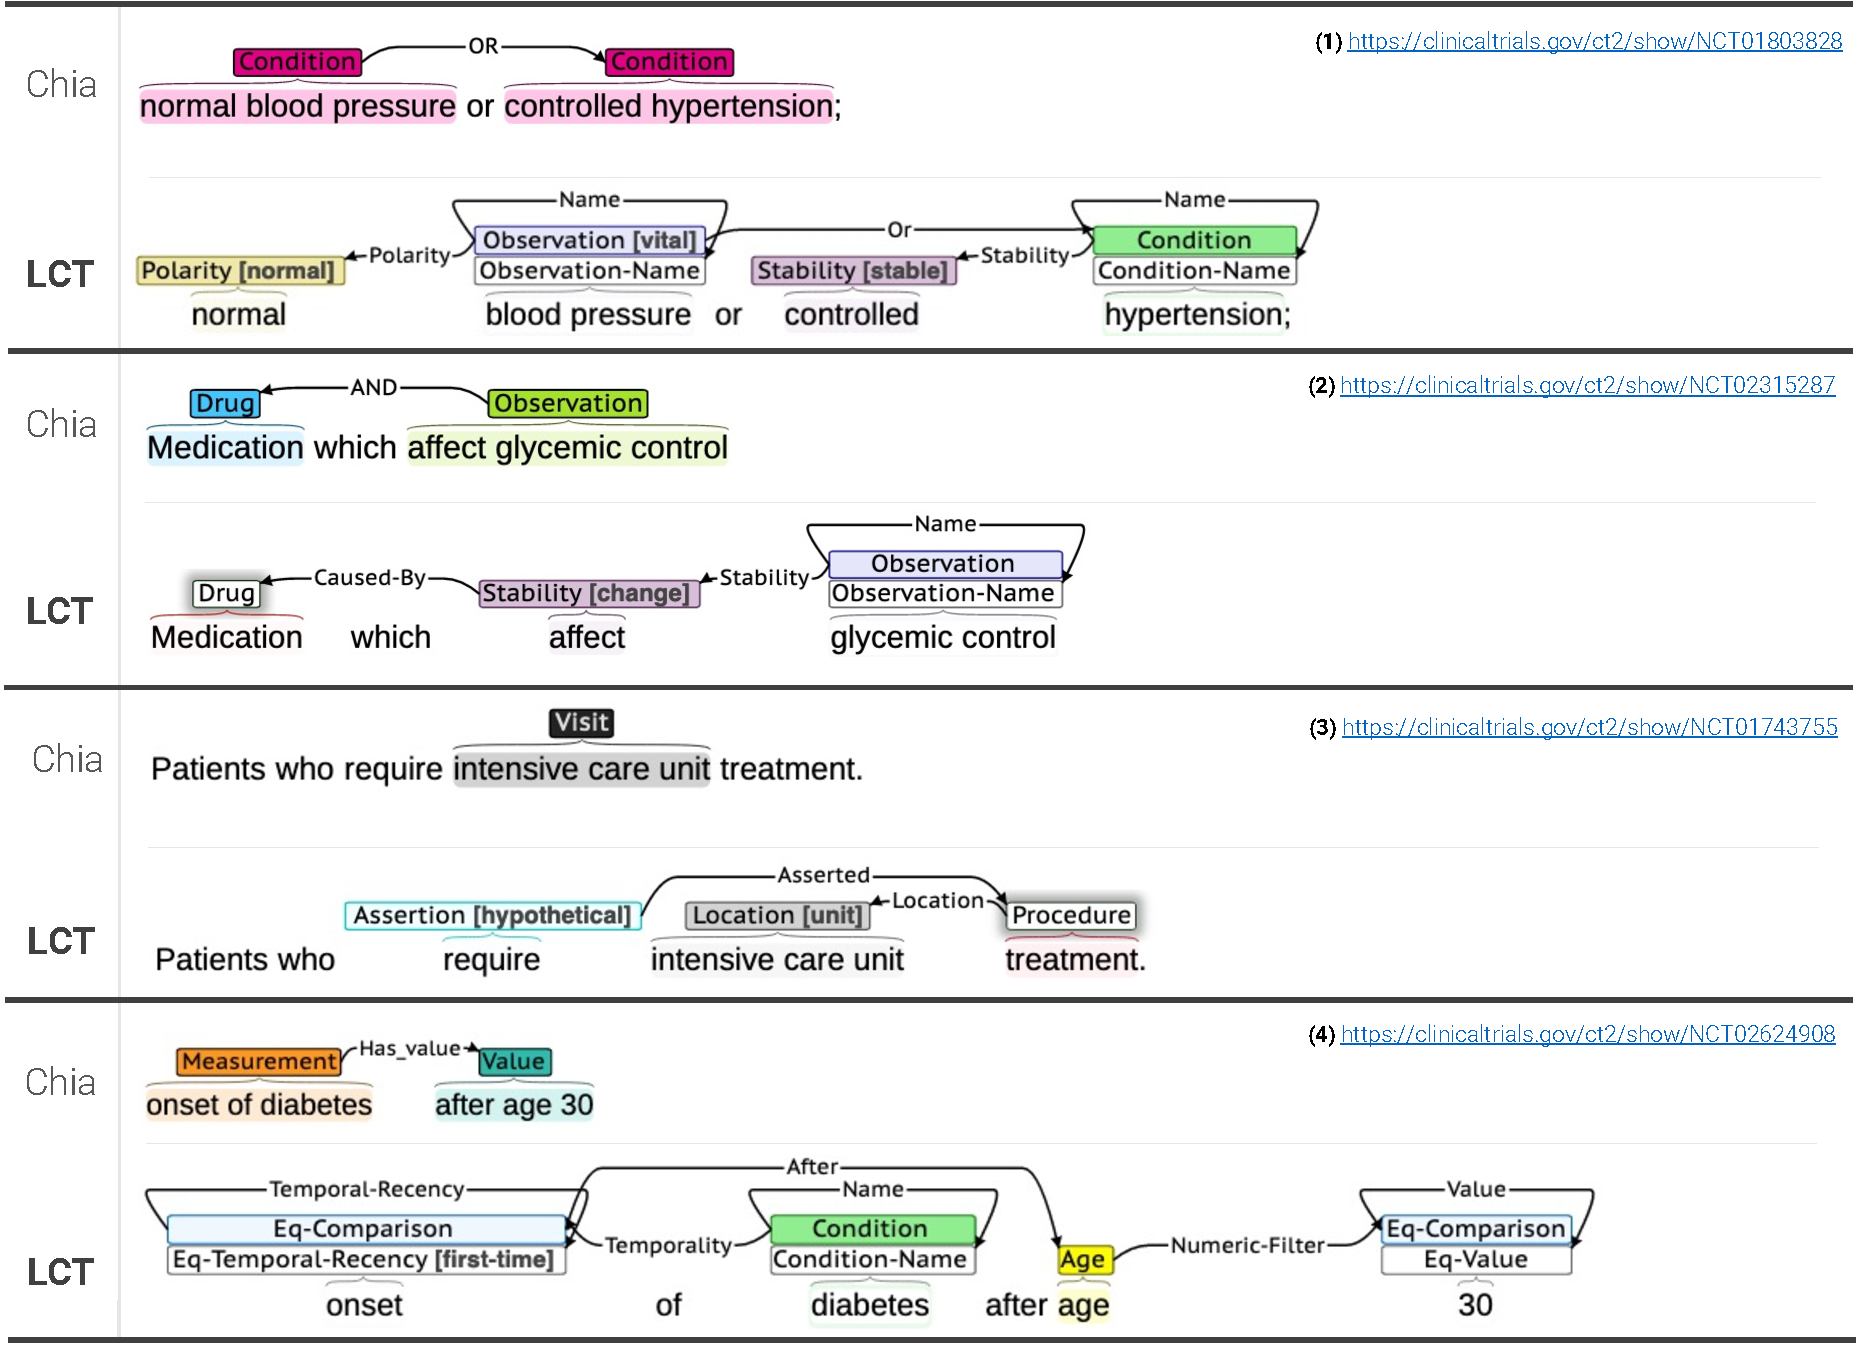
\includegraphics[scale=0.56]{Figures/Aim1/aim1_chia_vs_lct.pdf}  
    \caption{Examples of clinical trials eligibility criteria annotated with Chia and LCT annotation schemas. Each example shows a criterion from a Chia annotation (above) and an LCT annotation of the same text for purposes of comparison (below).}
    \label{aim1_fig_chia_vs_lct}
\end{figure}

\subsubsection{Annotation process}

We extracted 1,020 randomly selected clinical trials eligibility descriptions from \url{https://clinicaltrials.gov} from 2018 to 2021, 20 for training and inter-annotator comparison and 1,000 for post-training annotation. 

During annotation, 14 documents were found to be information poor (often with no spans to annotate) and discarded, resulting in 1,006 total annotated eligibility descriptions. Annotation was performed by two annotators, the first a biomedical informatician and the second a computer scientist. For initial annotation training, 20 documents were distributed to both annotators. Annotation was done in the following steps:

\begin{enumerate}
    \item Annotation meetings were held bi-weekly for 3 months following initial annotation training in which the annotation guidelines were introduced. Initial meetings focused on discussion of annotation guideline implementation and revision.
    \item After annotation guideline revisions and annotation training were completed, eligibility criteria were assigned to each annotator, with each clinical trial eligibility criteria annotated by a single annotator using the BRAT annotation tool \cite{stenetorp2012brat}. Due to differences in time availability for annotation, roughly 90\% (887 documents) of the annotation task was performed by the first annotator, and 99 documents by the second annotator.
    \item At the point in which 50\% of the corpus was annotated, we trained two neural networks (one for general entities and another for fine-grained entities) using the biLSTM+CRF-based NeuroNER tool \cite{dernoncourt2017neuroner} on our manually annotated eligibility criteria to predict annotations for the remaining 50\%.
    \item Manual annotation was completed on the remaining 50\% of eligibility descriptions by editing and correcting the predicted entities from NeuroNER in (3).

\end{enumerate}    
    
The resulting corpus included 887 single-annotated and 119 double-annotated total notes. Summary statistics for the corpus are shown in Table \ref{aim_1_tbl_corpora_compare}.

\begin{table}[h!]
\centering
  
\begin{tabular}{l|lll} 
 \toprule
 Measure & EliIE \cite{kang2017eliie} & Chia \cite{kury2020chia} & \textbf{LCT Corpus} \\
 \hline
    Disease domain & Alzheimer's Disease & All & \textbf{All} \\
    No. of Eligibility Descriptions & 230 & 1,000 & \textbf{1,006} \\
    No. of Annotations & 15,596 & 68,174 & \textbf{105,816} \\
    No. of Entity types & 8 & 15 & \textbf{50} \\
    No. of Relation types & 3 & 12 & \textbf{51} \\
    Mean Entities per doc. & - & 46 & \textbf{105} \\
    Mean Relations per doc. & - & 19 & \textbf{49} \\
 \hline
\end{tabular}

  \caption{\textbf{Annotation statistics for EliIE, Chia, and LCT corpora.}}
  \label{aim_1_tbl_corpora_compare}
\end{table}

\subsubsection{Inter-annotator agreement}
Inter-annotator agreement was calculated using F\textsubscript{1} scoring for entities and relations with 20 double-annotated documents. Entity annotations were considered matching only if entity types and token start and end indices matched exactly. Relations annotations were similarly considered matching only if relation type and token start and end indices of both the subject and target matched exactly.

Initial inter-annotator agreement using the 20 training documents was 76.1\% for entities and 60.3\% for relations. Inter-annotator agreement improved slightly to 78.1\% (+2\%) for entities and 60.9\% (+0.6\%) for relations in the 99 additional double-annotated documents, indicating reasonably high annotator agreement considering the complexity of the annotation task.

\subsubsection{Baseline prediction}
To evaluate baseline predictive performance on the LCT corpus, we first created a randomly assigned 80/20 split of the corpus, with 804 documents used for the training set and 202 for the test set. For entity prediction, we trained NER models using biLSTM+CRF and BERT \cite{devlin2018bert} neural architectures. For BERT-based prediction, we used two pretrained models trained on published medical texts, SciBERT \cite{beltagy2019scibert} and PubMedBERT \cite{gu2021domain}. For both biLSTM+CRF and BERT predictions, we trained one model to predict general entities and another for fine-grained entities. 

For relation extraction, we evaluated SciBERT for sequence classification as well as a modified BERT architecture, R-BERT, following methods developed by Wu \& He \cite{wu2019enriching}, also using the pretrained SciBERT model. Table \ref{aim1_tbl_hyperparams} shows hyperparameters used for each task.

\def\arraystretch{1.2}
\begin{table}[h!]
  \centering
  \def\arraystretch{1}
  \footnotesize
  \begin{tabular}{m{4cm} m{3cm} m{5cm} m{3cm}}
%\begin{table}
 \toprule
 \textbf{Task} & \textbf{Architecture} & \textbf{Hyperparameter / Embeddings} & \textbf{Training Value} \\
 \hline
    \multirow{4}{*}{\mbox{Named Entity Recognition}} &
    \multirow{4}{*}{\mbox{biLSTM+CRF}} 
    %Named Entity Recognition
        & Character Dimensions & 25 \\
        & & Token Embedding Dimensions & 100 \\
        & & Learning Rate & 0.005 \\
        & & Dropout & 0.5 \\
        & & Pretrained Embeddings & GloVe \cite{pennington2014glove} \\
    \hline
    \multirow{2}{*}{\mbox{Relation Extraction}} &
    \multirow{2}{*}{\mbox{BERT \& R-BERT}} 
        & Pretrained Model & SciBert  \\
        & & Learning Rate & 0.00003 \\
 \hline
\end{tabular}
  \caption{Hyperparameters and pre-trained embeddings used for named entity recognition and relation extraction baseline results. For the NER task, the same architecture and hyperparameters were used for both general and fine-grained entity models. For the relation extraction task, the same hyperparameters were used with both the BERT and R-BERT architectures.}
  \label{aim1_tbl_hyperparams}
\end{table}

We achieved the highest micro-averaged F\textsubscript{1} score of 81.3\% on entities using SciBERT and 85.2\% on relations using the R-BERT architecture with SciBERT \footnote{A full listing of baseline prediction results can be found with the annotation guidelines at \url{https://github.com/uw-bionlp/clinical-trials-gov-annotation/wiki/Named-Entity-Recognition-and-Relation-Extraction-performance}. }. Results of representative entities and relations are shown in Tables \ref{aim1_entity_f1} and \ref{aim1_relation_f1}.

\begin{table}[tp]
    \centering
    \def\arraystretch{1.4}
    \footnotesize
    \begin{tabular}{m{2cm} m{3.5cm} m{1.4cm} m{2.9cm} m{2.9cm} m{2.9cm}}
    \toprule
    \textbf{Category} & \textbf{Entity} & \textbf{Count} & \textbf{biLSTM+CRF} & \textbf{PubMedBERT} & \textbf{SciBERT} \\ \midrule
     & Condition & 7,087 & 78.6 / 78.1 / 78.3 & 76.1 / 79.4 / 77.7 & 78.4 / 83.3 / 80.8 \\
     & Contraindication & 142 & 93.7 / 78.9 / 85.7 & 77.4 / 80.0 / 78.6 & 100 / 96.6 / 98.3 \\
    Clinical & Drug & 1,404 & 76.8 / 81.3 / 79.0 & 74.1 / 80.9 / 77.4 & 73.4 / 80.9 / 77.0 \\
     & Encounter & 302 & 64.1 / 58.1 / 60.9 & 51.7 / 61.7 / 56.3 & 58.3 / 74.4 / 65.4 \\
     & Observation & 2,558 & 74.3 / 66.1 / 69.9 & 67.9 / 73.5 / 70.6 & 72.1 / 77.6 / 74.7 \\
     & Procedure & 3,016 & 68.4 / 75.5 / 71.9 & 67.0 / 75.9 / 71.2 & 71.3 / 79.4 / 75.1 \\
    \hline       
    \multirow{4}{*}[-4pt]{\mbox{Demographic}} & 
        Age & 708 & 91.3 / 95.4 / 93.3 & 82.4 / 88.5 / 85.3 & 99.1 / 98.3 / 98.7 \\
     & Birth & 27 & 100 / 80.0 / 88.8 & 100 / 62.5 / 76.9 & 100 / 62.5 / 76.9 \\
     & Death & 35 & 33.3 / 33.3 / 33.3 & 0.0 / 0.0 / 0.0 & 100 / 20.0 / 33.3 \\
     & Family-Member & 147 & 40.0 / 19.0 / 25.8 & 33.3 / 55.5 / 41.6 & 44.9 / 61.1 / 51.7 \\
     & Language & 194 & 92.5 / 96.1 / 94.3 & 73.8 / 100 / 84.9 & 96.6 / 93.5 / 95.0 \\
    \hline
    Logical & Negation & 952 & 74.3 / 82.7 / 78.2 & 60.9 / 73.1 / 66.4 & 73.5 / 82.9 / 77.9 \\
    \hline
    \multirow{6}{*}[-5pt]{\mbox{Qualifier}} &
        Assertion & 1,157 & 66.6 / 62.8 / 64.7 & 56.1 / 58.9 / 57.5 & 62.1 / 65.8 / 63.9 \\
         & Modifier & 3,464 & 65.0 / 58.3 / 61.5 & 59.2 / 64.0 / 61.5 & 58.5 / 65.4 / 61.8 \\
         & Polarity & 360 & 82.5 / 88.0 / 85.1 & 74.6 / 67.4 / 70.8 & 81.4 / 79.5 / 80.4 \\
         & Risk & 117 & 93.1 / 96.4 / 94.7 & 91.3 / 91.3 / 91.3 & 95.4 / 91.3 / 93.3 \\
         & Severity & 569 & 86.8 / 90.8 / 88.7 & 76.7 / 79.5 / 78.1 & 86.5 / 94.1 / 90.2 \\
         & Stability & 397 & 84.2 / 67.6 / 75.0 & 79.4 / 75.0 / 77.1 & 75.3 / 84.7 / 79.7 \\
    \hline
      &
        Criteria-Count & 33 & 50.0 / 66.6 / 57.1 & 28.5 / 40.0 / 33.3 & 12.5 / 20.0 / 15.5 \\
     & Eq-Comparison & 5,298 & 83.1 / 83.8 / 83.4 & 81.4 / 85.0 / 83.2 & 85.3 / 89.3 / 87.3 \\
     & Eq-Temporal-Period & 2,057 & 88.7 / 89.2 / 88.9 & 70.0 / 73.9 / 71.9 & 82.6 / 86.3 / 84.4 \\
     Comparative & Eq-Temporal-Recency & 131 & 68.7 / 84.6 / 75.8 & 43.4 / 55.5 / 48.7 & 50.0 / 66.6 / 57.1 \\
     & Eq-Temporal-Unit & 1,808 & 95.1 / 97.6 / 96.4 & 97.4 / 98.1 / 97.8 & 98.2 / 99.4 / 98.8 \\
     & Eq-Value & 3,835 & 91.8 / 95.3 / 93.5 & 95.5 / 96.2 / 95.9 & 96.4 / 97.1 / 96.7  \\
    \hline   
    Other &
        Location & 371 & 68.5 / 58.7 / 63.2 & 65.4 / 71.6 / 68.3 & 73.4 / 78.3 / 75.8 \\
    \hline
    - & Total & 56,146 & 80.2 / 79.6 / 79.9 & 75.3 / 78.7 / 77.0 & 79.0 / 83.7 / 81.3 \\
    
\end{tabular}
    \caption{\textbf{Baseline entity prediction scores (\%, Precision / Recall / F\textsubscript{1}).} Corpus-level micro-averaged scores are shown in the bottom row. For brevity a representative sample of entities is shown. \textit{Count} refers to the total count of unique spans annotated in the entire corpus. Entities included in the total count and scores but omitted for brevity are \textit{Acuteness, Allergy, Condition-Type, Code, Coreference, Ethnicity, Eq-Operator, Eq-Unit, Indication, Immunization, Insurance, Life-Stage-And-Gender, Organism, Other, Specimen, Study and Provider}.}
    \label{aim1_entity_f1}
\end{table}

\begin{table*}
    \centering
    \def\arraystretch{1.4}
    \footnotesize
    \begin{tabular}{m{3cm} m{3cm} m{2cm} m{3cm} m{3.7cm}}
\toprule
    \textbf{Category} & \textbf{Relation} & \textbf{Count} & \textbf{SciBERT} & \textbf{R-BERT+SciBERT} \\ \midrule
     & Abbrev-Of &           462 & 95.2 / 90.9 / 93.0 & 92.3 / 93.1 / 94.2 \\
    Alt. and Examples & Equivalent-To & 516 & 61.5 / 69.5 / 65.3 & 59.6 / 67.3 / 63.2 \\
     &                       Example-Of & 1,497 & 94.8 / 92.9 / 93.8 & 90.5 / 91.7 / 91.1 \\
    \hline
     &                       Contraindicates & 153 & 90.9 / 90.9 / 90.9 & 90.9 / 90.9 / 90.9 \\
     &                       Caused-By & 726 & 63.0 / 86.4 / 72.9 & 78.6 / 86.4 / 82.3 \\
     Clinical &              Found-By & 293 & 90.4 / 59.3 / 71.7 & 79.3 / 71.8 / 75.4 \\
     &                       Treatment-For & 457 & 69.2 / 69.2 / 69.2 & 61.7 / 74.3 / 67.4 \\
     &                       Using & 405 & 73.8 / 83.7 / 78.4 & 66.6 / 64.8 / 65.7 \\
    \hline
    \multirow{4}{*}[0pt]{\mbox{Logical}} & And & 821 & 54.1 / 60.0 / 56.9 & 53.8 / 53.8 / 53.8 \\
     &                       If-Then & 261 & 57.6 / 65.2 / 61.2 & 55.5 / 65.2 / 60.0 \\
     &                       Negates & 984 & 74.3 / 91.0 / 81.8 & 74.5 / 88.7 / 81.0 \\
     &                       Or & 4,156 & 85.1 / 93.2 / 89.0 & 88.4 / 92.2 / 90.2 \\
    \hline
     &               Asserted & 1,184 & 83.7 / 89.0 / 86.3 & 85.9 / 89.0 / 87.5 \\
     &                       Modifies & 3,400 & 90.9 / 94.2 / 92.5 & 92.2 / 95.4 / 93.8 \\
    Qualifier &               Risk-For & 90 & 92.3 / 85.7 / 88.8 & 92.8 / 92.8 / 92.8 \\
     &                       Severity & 529 & 80.2 / 96.6 / 87.6 & 86.3 / 96.6 / 91.2 \\
     &                       Stability & 395 & 76.0 / 92.6 / 83.5 & 76.4 / 95.1 / 84.7 \\
    \hline
    \multirow{6}{*}[-5pt]{Comparative} & After & 166 & 75.0 / 70.5 / 72.7 & 72.2 / 76.4 / 74.2 \\
     &                       Before & 320 & 70.2 / 86.6 / 77.6 & 78.1 / 83.3 / 80.6 \\
     &                       Duration & 243 & 59.3 / 79.1 / 67.8 & 64.5 / 83.3 / 72.7 \\
     &                       During & 350 & 66.6 / 68.7 / 67.6 & 63.6 / 65.6 / 64.6 \\
     &                       Numeric-Filter & 1,957 & 84.6 / 93.3 / 88.7 & 85.7 / 92.3 / 88.8 \\
     &                       Minimum-Count & 173 & 64.2 / 69.2 / 66.7 & 71.4 / 76.9 / 74.0 \\
     &                       Temporality & 2,645 & 80.7 / 90.7 / 85.4 & 81.8 / 92.2 / 86.7 \\
    \hline
    Other &                  Location & 207 & 64.2 / 94.7 / 76.6 & 69.2 / 94.7 / 80.0 \\
    \hline
    - & Total & 24,379 & 80.2 / 88.2 / 84.0 & 82.5 / 88.0 / 85.2
\end{tabular}
    \caption{\textbf{Baseline relation prediction scores (\%, Precision / Recall / F\textsubscript{1}).} Corpus-level micro-averaged scores are shown in the bottom row. For brevity a representative sample of relations is shown. \textit{Count} refers to the total count annotated in the entire corpus, including relations not shown. The count total excludes general to fine-grained entity relations, which as overlapping spans are not used for relation prediction. Relations included in the total count and scores but omitted for brevity are \textit{Acuteness, Code, Criteria, Except, From, Indication-For, Is-Other, Max-Value, Min-Value, Polarity, Provider, Refers-To, Specimen, Stage, Study-Of and Type}.}
    \label{aim1_relation_f1}
\end{table*}

\subsubsection{Annotation quality evaluation}
To determine the quality of single-annotated documents compared to those which were double-annotated, we trained NER models (one for general and another for fine-grained entities, as in earlier experiments) using SciBERT with the 887 single-annotated documents and evaluated on the 119 double-annotated documents. The results were a precision of 79.7\%, recall of 82.5\%, and an F\textsubscript{1} score of 81.4\%, which are very close to the highest performance of our randomly split train/test set results shown in Table \ref{aim1_entity_f1}. These results indicate relative uniformity and consistency in the corpus across both single- and double-annotated documents.

\def\arraystretch{1.2}
\begin{table}[h!]
\centering
\begin{tabular}{l l c c c}
 \toprule
 \textbf{Training Set} & \textbf{Test Set} & \textbf{Precision} & \textbf{Recall} & \textbf{F\textsubscript{1}} \\
 \hline
    Manual & Semi-automated & 75.4 & 82.1 & 78.6 \\
    Semi-automated & Manual & 80.1 & 79.9 & 80.0 \\
 \hline
\end{tabular}
\caption{\textbf{Results of NER experiments using the manually annotated and semi-automated portions of the corpus.} The manually annotated portion includes 513 documents while the semi-automatically annotated portion is 493 documents.}
\label{aim1_tbl_manual_semiauto}
\end{table}

As the latter near-half (493 documents) of the LCT corpus was automatically annotated, then manually corrected, we also evaluated the quality of the manually annotated portion versus the semi-automatically annotated portion to ensure consistency. We first trained NER models with SciBERT using the manually annotated portion and tested on the semi-automated portion, then reversed the experiment and trained on the semi-automated portion and tested on the manually annotated portion. Results are shown in Table \ref{aim1_tbl_manual_semiauto}.

Results of the experiments when training on both the manually and semi-automatically annotated halves of the corpus show comparable results, with the greatest difference being in precision, with the manual annotation-trained model performing slightly worse (-4.7\%) in prediction versus the semi-automated annotation-trained model. Overall F\textsubscript{1} scores were similar at 78.6\% and 80.0\%, suggesting reasonable consistency across the corpus.

\subsubsection{Limitations}
The LCT corpus is designed as a granular and robust resource of annotated eligibility criteria to enable models for entity and relation prediction as means of query generation. The corpus does have a number of limitations however which should be recognized. First, the corpus is largely singly annotated, with 119 of 1,006 documents (11\%) double annotated and reconciled, while double annotation is generally considered to be the gold standard in the NLP research community. However, the reasonably high F\textsubscript{1} score from experiments to evaluate NER when training on the singly annotated portion of the corpus suggests relative consistency of annotation across both single and double annotated documents. Additionally, entities in roughly half of the LCT corpus (493 documents) were automatically predicted, then manually corrected. This can potentially lead to data bias if predicted entities are not thoroughly reviewed and corrected by human annotators. Similar results from our experiments to detect differences in performance by training on the manually annotated portion versus the semi-automatically annotated portion (F\textsubscript{1} scores of 78.6\% and 80.0\%) suggest this may not be not a significant issue. \\

\subsubsection{Conclusion}
We created the LCT corpus, a gold standard human-annotated corpus of highly granular clinical trial eligibility criteria annotations. The NER and relation extraction models trained on this corpus achieved high performance and enable our subsequent aims.

\end{document}